\icode{E-MM-CA-L3-261014-001}
如图所示，在光滑水平地面上放置着一半径为 \(R\) 的 \(\frac{1}{4}\) 圆弧形滑块 \(B\)，其弧面光滑，在滑块 \(B\) 的右侧放置一连接有轻质弹簧的小球 \(C\)。现让小球 \(A\) 从滑块 \(B\) 的正上方距地面高 \(3R\) 处由静止释放，小球沿滑块 \(B\) 的切线进入圆弧面，然后从滑块 \(B\) 的末端水平滑出，之后小球 \(A\) 挤压弹簧但与弹簧未粘连。已知小球 \(A\) 的质量为 \(m\)，滑块 \(B\) 的质量为 \(2m\)，小球 \(C\) 的质量为 \(m\) 的 \(k\) 倍，重力加速度为 \(g\)。求：
\begin{enumerate}
	\item 小球 \(A\) 从滑块 \(B\) 末端滑出时，小球 \(A\) 和滑块 \(B\) 的速度分别为多少；
	\item 小球 \(A\) 挤压弹簧过程中，弹簧最大的弹性势能为多少；
	\item 要使小球 \(A\) 弹回后能追上滑块 \(B\)，求出 \(k\) 的取值范围。
\end{enumerate}

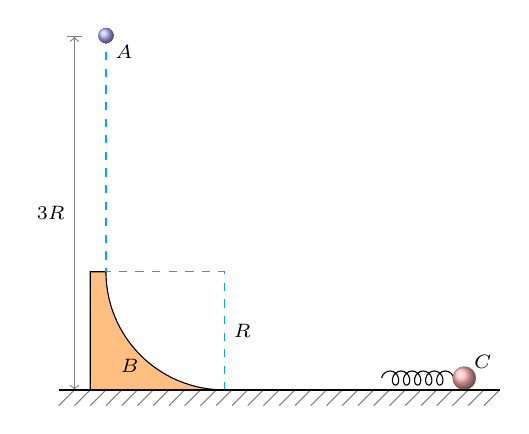
\begin{tikzpicture}[font=\scriptsize]
	\draw[fill=orange!50] (-.2,0)--(-.2,1.5)--(0,1.5) arc(180:270:1.5)--cycle;
	\draw[dashed,cyan] (0,4.5)--(0,1.5)--(1.5,1.5)--node[right,black]{\(R\)}(1.5,0);
	\shade[ball color=blue!30] (0,4.5)node[below right]{\(A\)} circle(.1);
	\draw[<->|,gray] (-.4,0)--node[left,black]{\(3R\)}(-.4,4.5);
	\draw[decoration={aspect=.8,segment length=4,amplitude=.9mm,coil},decorate] (3.5,.15)--(4.5,.15);
	\shade[ball color=red!30] (4.55,.15)node[above right]{\(C\)} circle(.15);
	\foreach \x in {-.6,-.4,...,5}
		\draw[gray] (\x,-.2)--++(.2,.2);
	\draw[thick] (-.6,0)--(5,0);
	\node at(.3,.3){\(B\)};
\end{tikzpicture}
\begin{answer}
   （）\(v_A = 2 \sqrt{gR}\)，水平向右；\(v_B = \sqrt{gR}\)，水平向左（2）\(E_{pm} = \frac{2kmgR}{k + 1}\)（3）\(k > 3\)\qquad 提示：反冲模型、类碰撞模型 
\end{answer}